\documentclass[11pt]{report}
\usepackage{geometry, graphicx, kotex, imakeidx, titlesec, array} % necessary packages
\usepackage{mathptmx}   
\usepackage{amsmath, amsthm, amssymb, mathrsfs, multirow, verbatim} % supplementary packages
\usepackage[nobiblatex]{xurl} % enable linebreak of \url command
\usepackage{indentfirst} % force indentation at every first paragraph of chapters, sections and subsections
\usepackage{booktabs} % table tool
\usepackage{ragged2e}
\usepackage{setspace}
\usepackage{natbib}
%\usepackage{algorithm2e}
\usepackage{algorithm}
\usepackage{algpseudocode}
%%%\usepackage[style=apa,backend=biber]{biblatex}
%%%\addbibresource{references.bib}

\geometry{letterpaper, left=25mm, right=25mm, top=25mm, bottom=25mm}  % set the paper size and the margins
  
\titleformat{\chapter}{\normalfont\LARGE\bfseries}{\chaptertitlename\ \thechapter.}{10pt}{\Large} % chapter style
\newtheorem{theorem}{Theorem} % theorem environment
\newtheorem{definition}{Definition} % definition environment
% if you need similar environments like lemma, corollary or remark, add them all.
\makeindex % command for making an index chapter

\linespread{1.5} % set the vertical spacing between successive lines (the ratio of the maximal height of a normal font and the base lineskip)

\renewcommand\arraystretch{1.3} % increase the vertical spacing by 30%

%%% stands for a new chapter or a new page
%% stands for a new section
% stands for a comment

%%%%
%\input{macros}

\begin{document}

\newpage 
\begin{center}
\huge Testing a Modern Inference Framework for POMP Models: A Case Study Using Stochastic Volatility  
\par\vspace{1cm} % spacing can be adjusted
\begin{figure}[ht]
\begin{center}

\includegraphics[width=.4\textwidth]{umichlogo.png}
\end{center}
\end{figure}
{\fontsize{16pt}{16pt}\selectfont by \par Dae Hyun Kim \par} % put the student's name here
\vspace{1.0cm}
\par\vspace{0.2cm}
{\fontsize{14pt}{14pt}\selectfont Supervisor Professor: Edward Ionides \par}
\vspace{0.1cm}
\par\vspace{0.2cm}
{\fontsize{14pt}{14pt}\selectfont Graduate Student Mentor: Aaron Abkemeier \par}
\vspace{0.7cm}
\vspace{10pt}
{\fontsize{16pt}{16pt}\selectfont Department of Statistics \par }  % You can reduce the character spacing to make the department name on one line. If it takes up more than two lines, please reduce the vertical spacing after the title appropriately.
\vspace{1.5cm}
{\fontsize{16pt}{16pt} University of Michigan\par} 
\vspace{1cm}
{\fontsize{14pt}{14pt}\selectfont April 2025}
\end{center}

\newpage 
\pagenumbering{roman} % set the page number as roman type from this page on.
\newgeometry{left=30mm, right=30mm, top=30mm, bottom=30mm} % set the paper size and the margins
% Margins shall be changed to bottom and top 3 cm, right and left 2 cm from this page forward.
\addcontentsline{toc}{chapter}{Abstract}
\begin{center}
\par\vspace{20pt}
\large \textbf{Abstract}
\end{center}

\normalsize
\justifying % this command available with \usepackage{ragged2e}
\doublespacing
The \textbf{pypomp} package is a new Python-based library for modeling likelihood-based inference on partially observed Markov process (POMP) models. Designed with the same goals as the R package \textbf{pomp}, \textbf{pypomp} offers a flexible environment for modeling nonlinear, non-Gaussian dynamic systems and supports both standard particle filtering and gradient-based estimation methods. By leveraging modern computational tools such as automatic differentiation (AD) and Graphics Processing Unit (GPU) acceleration via JAX, \textbf{pypomp} enables efficient inference for POMP models. We test and validate the \textbf{pypomp} package by using the Heston stochastic volatility model as a test case. Through this case study, we indicate the potential of \textbf{pypomp} to serve as a robust, extensible tool for scientific modeling and the development of advanced inference algorithms.
\par

\par\vspace{20pt}
%\textbf{Keywords}: iterated filtering, automatic differentiation, stochastic volatility

\newpage


%%% table of contents
\renewcommand*\contentsname{Table of Contents}
\addcontentsline{toc}{chapter}{Table of Contents}
\tableofcontents

\bigskip


%%% first chapter of the main body

\chapter{Introduction}\label{chap:intro}
\pagenumbering{arabic} % set the page number as Arabic type from this page on.
Inference for dynamic systems governed by latent processes is a core process in modern statistical science, with applications to various fields such as epidemiology, ecology, and finance. Partially observed Markov process (POMP) models, also known as hidden Markov models or state space models provide a principled framework for modeling such systems, in which a latent stochastic process drives an observed time series. However, only partial and noisy observations of the true underlying state are available in POMP models and general Maximum Likelihood Estimation (MLE) is often infeasible due to the intractability of the likelihood, which involves integrating over high-dimensional latent state spaces. 


The improved Iterated Filtering (IF2) algorithm introduced by \citet{ionides2015inference}, suggests an alternative to approach these challenges. IF2 uses the particle filter, also known as the sequential Monte Carlo (SMC) method, to estimate parameters in POMP models and it iteratively refines parameter estimates by introducing stochastic perturbations to the parameters, which facilitates convergence to the MLE. IF2 is a plug-and-play method that enables parameter estimation without requiring analytic expressions for transition densities, making it applicable to a wide variety of scientific models such as epidemiology 
\citep{subramanian2021quantifying}, \citep{wheeler2024informing}, \citep{king2008inapparent}, ecology \citep{li2024inference}, and finance \citep{szczepocki2020application}, \citep{sunmodel}.


The R package \textbf{pomp} has provided a powerful framework including IF2 for likelihood-based inference on POMP models \citep{king2016statistical}, but with the growing use of Python in scientific computing, there is a need for a library with similar modeling capabilities that also support modern numerical frameworks. In response to these needs, the \textbf{pypomp} package is being developed as a Python-based analog to \textbf{pomp}, and it supports plug-and-play particle filtering and simulation for POMP models, but it is also designed as a library for new algorithmic development. Key innovations in \textbf{pypomp} include the use of automatic differentiation (AD) for efficient gradient computation and the integration of JAX for just-in-time (JIT) compilation and GPU acceleration, enabling significant computational efficiency. One of the central algorithmic contributions of \textbf{pypomp} is the Iterated Filtering with Automatic Differentiation (IFAD) algorithm, introduced by \citet{tan2024accelerated}. Unlike IF2, which relies on stochastic perturbations for optimization, IFAD integrates gradient based updates through AD. This approach improves computational efficiency by combining rapid exploration of the parameter space via stochastic perturbations with precise gradient refinement. However, as \textbf{pypomp} is currently at early stages of development, it requires rigorous testing to ensure its correctness, stability, and reproducibility across applications.


We evaluate and test the current state of \textbf{pypomp} by using the Heston stochastic volatility model as a diagnostic benchmark. \citet{sunmodel} applied the IF2 algorithm using the \textbf{pomp} package in R to estimate the parameters of the Heston stochastic volatility model and we attempted to replicate these results using IF2 in \textbf{pypomp}. We then apply IFAD within the \textbf{pypomp} framework to estimate the same model parameters, comparing the inference quality, stability, and computational efficiency. Rather than focusing on improved inference for the Heston model itself, this research uses the model as a structured test case for evaluating the behavior and correctness of \textbf{pypomp}. 


Our contributions extend beyond benchmarking by helping \textbf{pypomp} to advance through rigorous testing and debugging. Specifically, we identified several critical issues and provided concrete fixes and analysis that contribute to the development of a robust, reliable inference in \textbf{pypomp}. As \textbf{pypomp} is currently in pre-release, our numerical results indicate its potential for development and provide insights as an innovative library for scientific inference and methodological research in dynamic systems.


%%%  the second chapter of the main body
\chapter{Background}\label{chap:background}

\section{Iterated Filtering Algorithms}
The key idea behind IF2 is to embed the estimation of parameters within a particle filter by introducing small random perturbations to the parameters across time steps. These perturbations are gradually reduced over multiple iterations, enabling the algorithm to stochastically explore the likelihood surface and converge toward the MLE. Unlike its predecessor, IF1 introduced by \citet{ionides2011iterated}, which approximates the score function via conditional moments, IF2 performs an iterated Bayes map, providing more robust numerical properties and convergence guarantees. (pseudocode in Appendix A)

The particle filter is a foundational tool for inference in POMP models. It enables likelihood-based inference \citep{ionides2006inference} and Bayesian inference \citep{chopin2013smc2}, \citep{andrieu2010particle} by providing Monte Carlo estimates of the likelihood function of observed data given model parameters. Specifically, the particle filter approximates the likelihood by simulating a collection of possible latent trajectories (particles) and sequentially weighting them according to how well they explain the observed data. This approach is both flexible and powerful, particularly for models where the latent dynamics are nonlinear and non-Gaussian \citep{arulampalam2002tutorial}, \citep{kitagawa1987non}. On top of that, the particle filter produces an unbiased estimate of the likelihood \citep{doucet2001sequential}, making it suitable for likelihood-based inference as it only requires accurate estimates for the likelihood. As a result, IF2 builds directly on the particle filter to perform plug-and-play likelihood maximization, without losing the statistical rigor of likelihood-based approaches.


The advantages of IF2 are its plug-and-play flexibility and stochastic robustness. Specifically, IF2 does not require the evaluation of transition densities, which allows it to be applied to models defined via simulation and the iterative perturbation process helps avoid early convergence to the local optima, which is common in complex likelihood surfaces. Also, the numerical results from \citet{ionides2015inference} indicate that IF2 can approximate the MLE arbitrarily well, under mild regularity conditions, as the number of particles and iterations increase.


The original implementation of IF2 was developed in the R package \textbf{pomp}, but R presents limitations in computational scalability, especially for models requiring GPU acceleration or AD. This is where Python and \textbf{pypomp} become critically useful. The field of Python research has grown rapidly due to its integration with high-performance libraries like JAX, as well as GPU-accelerated frameworks. As \textbf{pypomp} leverages modern features such as JIT compilation and AD, it makes it particularly well-suited for research using large-scale data.




\section{Automatic Differentiation Particle Filter}
Automatic differentiation (AD) is a computational process that enables the efficient and accurate calculation of derivatives for functions implemented as computer programs. Also, AD computes exact derivatives by systematically applying the chain rule to a sequence of elementary operations \citep{rall1996introduction}, \citep{verma2000introduction}. This capability is particularly powerful in fields such as machine learning, numerical optimization, and scientific computing, where gradient based methods are used.

AD operates by breaking down a function into a finite sequence of elementary operations and computing their derivatives step-by-step. AD can be implemented in two primary modes:
\begin{enumerate}
    \item \textbf{Forward Mode}:
    \begin{itemize}
        \item Computes derivatives by propagating derivatives from the inputs to the outputs.
        \item Efficient for functions with few inputs and many outputs.
    \end{itemize}
    \item \textbf{Reverse Mode}:
    \begin{itemize}
        \item Computes derivatives by propagating gradients backwards from the outputs to the inputs.
        \item Efficient for functions with many inputs and few outputs.
    \end{itemize}
\end{enumerate}
Both modes rely on the chain rule to propagate derivatives through computation:
\[\frac{\partial f}{\partial x} = \frac{\partial f}{\partial y} \cdot \frac{\partial y}{\partial x}\]

Recent work has extended the use of AD to particle filtering and inference for POMP models. The advantage of using AD is the gradient-based optimization for POMP models. Several papers have explored differentiable particle filters. For instance, \citet{jonschkowski2018differentiable} introduced differentiable filtering networks, and \citet{naesseth2018variational} proposed variational inference approaches using AD to optimize latent state models. However, these early approaches typically relied on low variance but asymptotically biased estimators of the gradient, raising concerns about their long-term reliability and statistical guarantees.

The Automatic Differentiation Particle Filter (ADPF), introduced by \citet{tandifferentiable}, overcomes these issues by framing the particle filter as a differentiable computational graph. On top of that, \citet{tan2024accelerated} introduces the Measurement Off-Parameter with discount factor $\alpha$ (MOP-$\alpha$) algorithm (pseudocode in Appendix A) that defines estimators for the gradient of the log-likelihood where the estimators balance the tradeoff between bias and variance. At $\alpha = 0$, low-variance estimators can be highly biased, while at $\alpha = 1$, unbiased estimators tend to suffer from high Monte Carlo variability. MOP-$\alpha$ interpolates between these extremes, allowing users to refine the factor based on precision needs.

The Iterated Filtering with Automatic Differentiation (IFAD) algorithm (pseudocode in Appendix A) introduced by \citet{tan2024accelerated} represents another development of using ADPF. The IFAD algorithm incorporates MOP-based gradient estimators into the structure of the IF2 algorithm. Like IF2, IFAD executes a stochastic perturbation of parameters through a particle filter. However, instead of fully relying on perturbations to update parameter estimates, IFAD supplements this process with gradient-based updates using AD. This process enables IFAD to overcome the two core challenges of IF2 such as Monte Carlo variability from noisy perturbation updates and slow convergence in high-dimensional spaces.

\section{Stochastic Volatility Models}
Stochastic volatility models play a central role in financial modeling, where accurately capturing the evolution of asset price variability is crucial for derivative pricing, risk management, and portfolio allocation. Among these models, the Heston model is widely used due to its ability to represent volatility as a mean-reverting stochastic process. However, parameter estimation for such models is challenging because of the intractability of their likelihood functions and the presence of latent variables.

The estimation of parameters in stochastic volatility models remains a challenging problem, primarily due to the computational complexity of the likelihood function, which involves high dimensional integration. Various methods have been developed to address these challenges. \citet{ait2007maximum} developed a maximum likelihood estimation method that addresses these challenges by employing closed-form approximations to the likelihood function. \citet{chib2002markov} and \citet{chib2006analysis} developed Markov Chain Monte Carlo (MCMC) algorithms for generalized stochastic volatility models. However, these methods are computationally intensive for high dimensions.

%Volatility is a measure of the variability or uncertainty of asset prices, and it is a fundamental concept in finance. The modeling of volatility is crucial for applications such as option pricing and risk management. Traditional models, such as the Black-Scholes model from \textbf{\citet{black1973pricing}, assume constant volatility over time. However, the evidence from financial markets such as volatility smile \textbf{\citet{derman1994riding} has shown that volatility is not constant but varies over time and traditional models often fail to reflect real-world dynamics. This has implied the development of stochastic volatility models and volatility started to get regarded as a stochastic process. 

The Heston model introduced by \citet{heston1993closed}, one of the most widely used stochastic volatility models includes a mean-reverting stochastic process for volatility, revealing the limitations of constant volatility models. Specifically, it assumes that the variance of asset returns follows a Cox-Ingersoll-Ross (CIR) process, expressed as:
\[d\nu_t = \kappa(\theta - \nu_t) \, dt + \xi \sqrt{\nu_t} \,dW_t^\nu\]
where 
\begin{itemize}
    \item $\nu_t$ is the instantaneous variance of the asset price at time $t$,
    \item $\kappa$ is the rate of mean reversion in variance, 
    \item $\theta$ is the long-term mean level of variance ($\lim_{t \to \infty} \mathbb{E}[\nu_t] = \theta$),
    \item $\xi$ is the volatility of the volatility,
    \item $W_t^\nu$ is the Wiener process in the volatility,
\end{itemize}
Simultaneously, the asset price $S_t$ changes according to the following stochastic differential equation:
 \[dS_t = \mu S_t\, dt + \sqrt{\nu_t} S_t \, dW_t^S\] 
 where:
\begin{itemize}
\item $S_t$ is the asset price at time $t$,
\item $\mu$ is the average growth rate of the asset price 
\item $W_t^S$ is the Wiener process in the asset price
\end{itemize}
 
The Heston model provides a realistic framework for understanding how volatility changes over time, enabling more accurate pricing of financial instruments and better investment decisions with market uncertainty. Therefore, it is effective for testing and comparing parameter estimation algorithms, such as the IF2 algorithm and the IFAD algorithm.
\newpage

\chapter{Debugging pypomp}\label{chap:debugging}
As part of evaluating IF2 and IFAD implementations in the \textbf{pypomp} package, we encountered several numerical instabilities and inconsistencies while testing the Heston stochastic volatility model. These issues motivated a deeper investigation into the underlying mechanics of \textbf{pypomp} and led to insights critical to the future reliability of the package.

\section{Original Testing}
From the outset, the \textbf{pypomp} organization incorporated a system of unit tests designed to ensure that core functionalities such as particle simulation, likelihood computation, and filtering are not broken when changes are made to the code. On top of that, unit tests provide early warnings if numerical results shift unexpectedly due to subtle changes in implementation, such as modifications to random number handling or model setup. This unit testing framework greatly aided the debugging process by allowing us to localize problems quickly when inconsistencies were observed during benchmarking.
In addition to unit testing, IF2 and the particle filter in \textbf{pypomp} were evaluated through performance benchmark tests called quantitative tests, or simply quant tests, named by the \textbf{pypomp} organization. Unlike unit tests, quant tests measure the time to complete filtering and optimization tasks, the memory requirements during computation, and the number of iterations needed to achieve convergence for a maximization algorithm. The quant tests were performed using Linear Gaussian model and Dhaka cholera model. The Linear Gaussian model offers an analytically tractable benchmark, where exact likelihoods and parameter estimates are known. Since the Kalman filter provides the exact optimal inference for this model, deviations in \textbf{pypomp} results could be precisely identified and quantified, making it an ideal diagnostic tool for basic functionality and performance. The Dhaka cholera model introduced by \citet{king2008inapparent} represents a complex, nonlinear, epidemiological system. By using this model, it allowed developers to assess scalability to large datasets, robustness under complex latent dynamics with the particle filter and IF2 algorithm. Performance metrics from these two models helped ensure that IF2 and particle filter in \textbf{pypomp} could handle both analytically simple and scientifically realistic POMP models with reasonable computational resources.

\section{Issue in Original R code}
Before investigating issues within \textbf{pypomp} itself, we first carefully examined the R code provided by \citet{sunmodel} for the Heston stochastic volatility model. During this process, we identified a critical flaw that the latent volatility process $V$ was not correctly updated over time inside the rprocess simulation step.

In the correct implementation of the Heston model, volatility $V$ must evolve dynamically according to its stochastic differential equation. However, in the original R code, it did not update $V$ from one time step to the next. As a result, volatility remained constant or evolved incorrectly, fundamentally altering the latent dynamics of the model. We corrected this by adding a proper stochastic update for $V$ at each time step within the rprocess function in R. 

\section{Initial Value Perturbation Issue in Iterative Filtering}
The first major issue was discovered when we were analyzing parameter evolution during IF2 optimization. In the R pomp package, initial value parameters (IVPs) such as the initial state of the latent process are only perturbed during the first filtering iteration, reflecting the fact that IVPs lose their influence over time as the latent process evolves \citep{ionides2015inference}, \citep{king2016statistical}. Perturbing IVPs throughout the entire optimization adds unnecessary noise and destabilizes the inference. By contrast, \textbf{pypomp} initially perturbed IVPs continuously across all iterations as it did not distinguish IVPs from other parameters in the IF2 process, which reduced optimization performance and introduced instability to our numerical results. This misbehavior was subsequently corrected by Jun Chen, one of the founding developers in the \textbf{pypomp} organization. 


Even after the IVPs issue was resolved, the log-likelihood estimates obtained using 1000 particles were significantly below the expected value (around 11849, based on \citet{sunmodel}’s results) and often produced errors. However, when using 10,000 particles, the estimated log-likelihood reached the expected value and errors disappeared.

\section{Particle Depletion Assumption}
This pattern suggested the presence of particle depletion, also known as particle degeneracy, a common problem in particle filter algorithms. Particle depletion occurs when, after resampling, most particles are either discarded or receive extremely low weights \citep{daum2011particle}. This leads to a lack of diversity in the particle population and log-likelihood estimates become biased or undefined as likelihood estimates are computed from weighted particles \citep{gustafsson2002particle}. Also, when estimating parameters in IF2, if particles get depleted early, the algorithm struggles to explore different parameter values, resulting in suboptimal estimates. To mitigate particle depletion, increasing the number of particles reduces variance and prevents all weights from collapsing, so the numerical stability gets improved. As the characteristics of particle depletion correspond to the situations that we were experiencing, it supported our assumptions.


To diagnose this, we analyzed the conditional log-likelihoods and particle traces of parameters. In a POMP model, the observations are random, and we want to compute the likelihood of observing the data, given a parameter $\theta$. Instead of looking at the full likelihood at once, we break it down sequentially. At each time point $t_k$, the conditional likelihood is the probability density of the current observation, given all previous observations. In other words, the conditional log-likelihood is the value of the density of $Y(t_k) \mid Y(t_1), \dots, Y(t_{k-1})$ evaluated at $Y(t_k) = y_k^*$ where $ Y(t_k)$ is the observable process, and $y_k^*$ is the data, at time $t_k$.

Thus, the conditional log-likelihood at time $t_k$ is
\[
\ell_k(\theta) = \log f\left[Y(t_k) = y_k^* \mid Y(t_1) = y_1^*, \dots, Y(t_{k-1}) = y_{k-1}^*\right]
\]
where $f$ is the probability density above.

If particles are depleted at some time $t_k$, meaning most particle weights are near $0$ except for very few, then the sum of the weights becomes very small. This will affect the conditional log-likelihood $\ell_k(\theta)$ to be highly negative and it will show a large negative spike in the plot. In contrast, when particles are not struggling from depletion, $\ell_k(\theta)$ behaves smoothly without huge fluctuations.
\begin{figure}[ht] 
\begin{center}
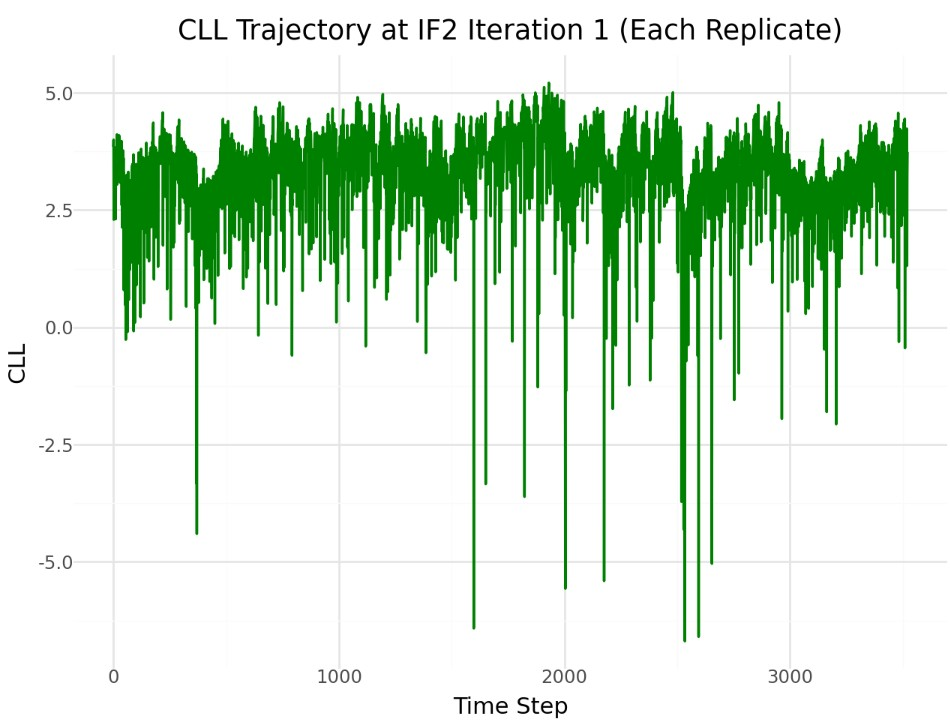
\includegraphics[width=\textwidth]{rep1.jpg}
\end{center}
\caption{Conditional Log-likelihood}
\label{fig:cllplot}
\end{figure}

\newpage
Figure 3.1 represents that the conditional log-likelihood is calculated smoothly as sudden sharp drops in $\ell_k(\theta)$ over time is not identified.


During IF2, the parameters are perturbed at each time point $t_k$ slightly and each particle carries a slightly perturbed parameter $\theta_k^{(i)}$. The particle traces of parameters record $\theta_k^{(i)}$ for each particle $i$ over each time $t_k$, so tracking particle traces is helpful to analyze Whether parameters collapse (particles become identical), or the particle diversity is maintained. Thus, if a particle depletion occurred, then most particle traces will collapse to a few lines and the spread in parameter values will be lost.

%\begin{figure}[ht] 
%\begin{center}
%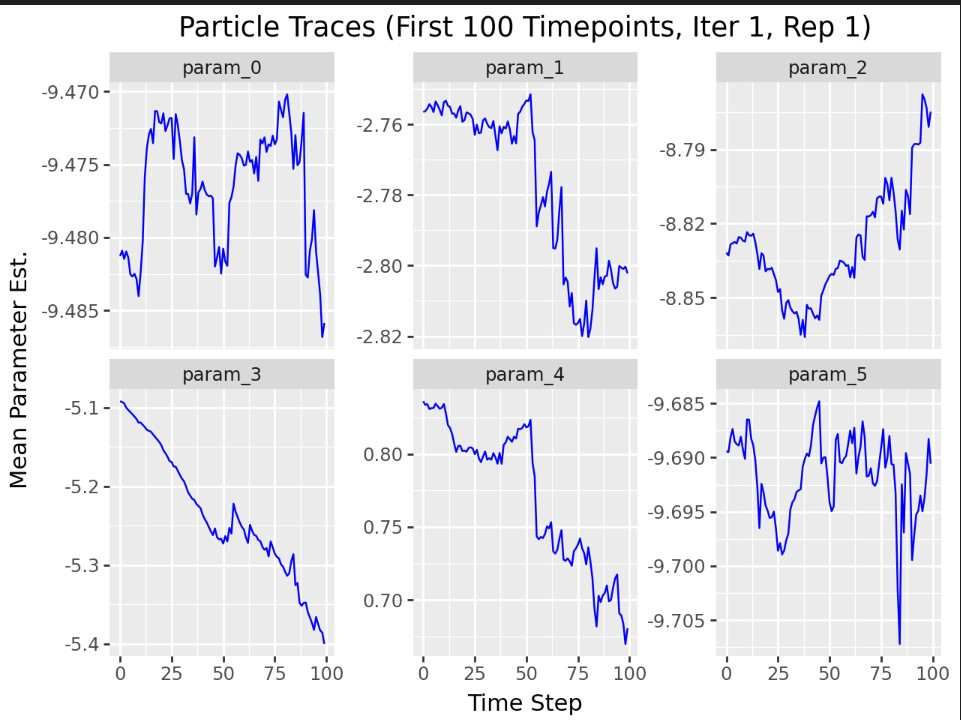
\includegraphics[width=\textwidth]{iter1rep1.jpg}
%\end{center}
%\caption{Particle Trace}
%\label{fig:ptraceplot}
%\end{figure}

By inspecting these traces, we attempted to localize potential failures at particular time points. However, no obvious collapse or degeneration was observed across the traces, suggesting the problem might lie elsewhere.

\section{Just-in-time Compilation Issue}
A deeper debugging and investigation revealed that the root cause of instability and errors was not particle depletion, but rather faulty random number generation during JIT compilation. Specifically, random perturbations for particles were originally drawn using np.random.normal, a NumPy function. JAX's JIT compilation requires that all random number generations be explicitly managed via jax.random.PRNGKey because JAX uses pure functional programming while NumPy does not. Previously, keeping keys from being split and mixing np.random with JIT-compiled functions led to uncontrolled randomness. In other words, the same random values were reused repeatedly across particles and iterations, corrupting the filtering and optimization process and producing errors in likelihood estimations. After using JAX random number generation such as jax.random.normal rather than np.random and ensuring that keys were explicitly split, the random perturbations became truly random, the errors disappeared, and likelihood estimates stabilized.


\chapter{Iterative Filtering in pypomp}\label{chap:pypompif2}
\citet{sunmodel} applied the IF2 algorithm implemented in the R package \textbf{pomp} to estimate the parameters of the Heston stochastic volatility model using daily S$\&$P500 log-return data from 2010 to 2024. His study indicated the ability of IF2 to recover volatility dynamics consistent with market benchmarks like the VIX index, and showed the model significantly outperformed classical GARCH-based benchmarks in terms of log-likelihood. His research also conducted profile likelihood estimation on each parameter, initially profiling over $\mu$, and subsequently fixing $\mu$ at its smoothed profile MLE to improve optimization stability. In our study, we sought to replicate Sun’s results using the \textbf{pypomp} package. While Sun performed profiling to construct confidence intervals, we did not require profiling of $\mu$ in our setting since our goal was not to conduct inference but to test and validate the numerical behavior of the \textbf{pypomp} IF2 implementation. 
%%

%%
\section{Log-likelihood Trace}\label{sec:ll_trace}
The log-likelihood trace records the IF2 log-likelihood estimate at each iteration. It is computed using perturbed parameters and is noisy, but the trend should generally increase (or negative log-likelihood should decrease). This is an internal measure during optimization progress, and it indicates whether IF2 is improving the model fit during iterative process.

To evaluate the internal optimization process of both \textbf{pomp} and \textbf{pypomp}, we compared the log-likelihood values estimated at each iteration of the IF2 algorithm. To ensure that differences in starting points did not affect the comparison, we sampled and stored 120 initial parameter sets from \citet{sunmodel}'s model using \textbf{pomp} and then used exactly the same starting values when running IF2 optimization in our model using \textbf{pypomp}. This guarantees that IF2 of both \textbf{pomp} and \textbf{pypomp} implementations began from identical initial conditions, allowing us to attribute any differences to algorithmic behavior rather than random initial variability.
%\newpage
%\bigskip
\begin{figure}[ht] 
\begin{center}
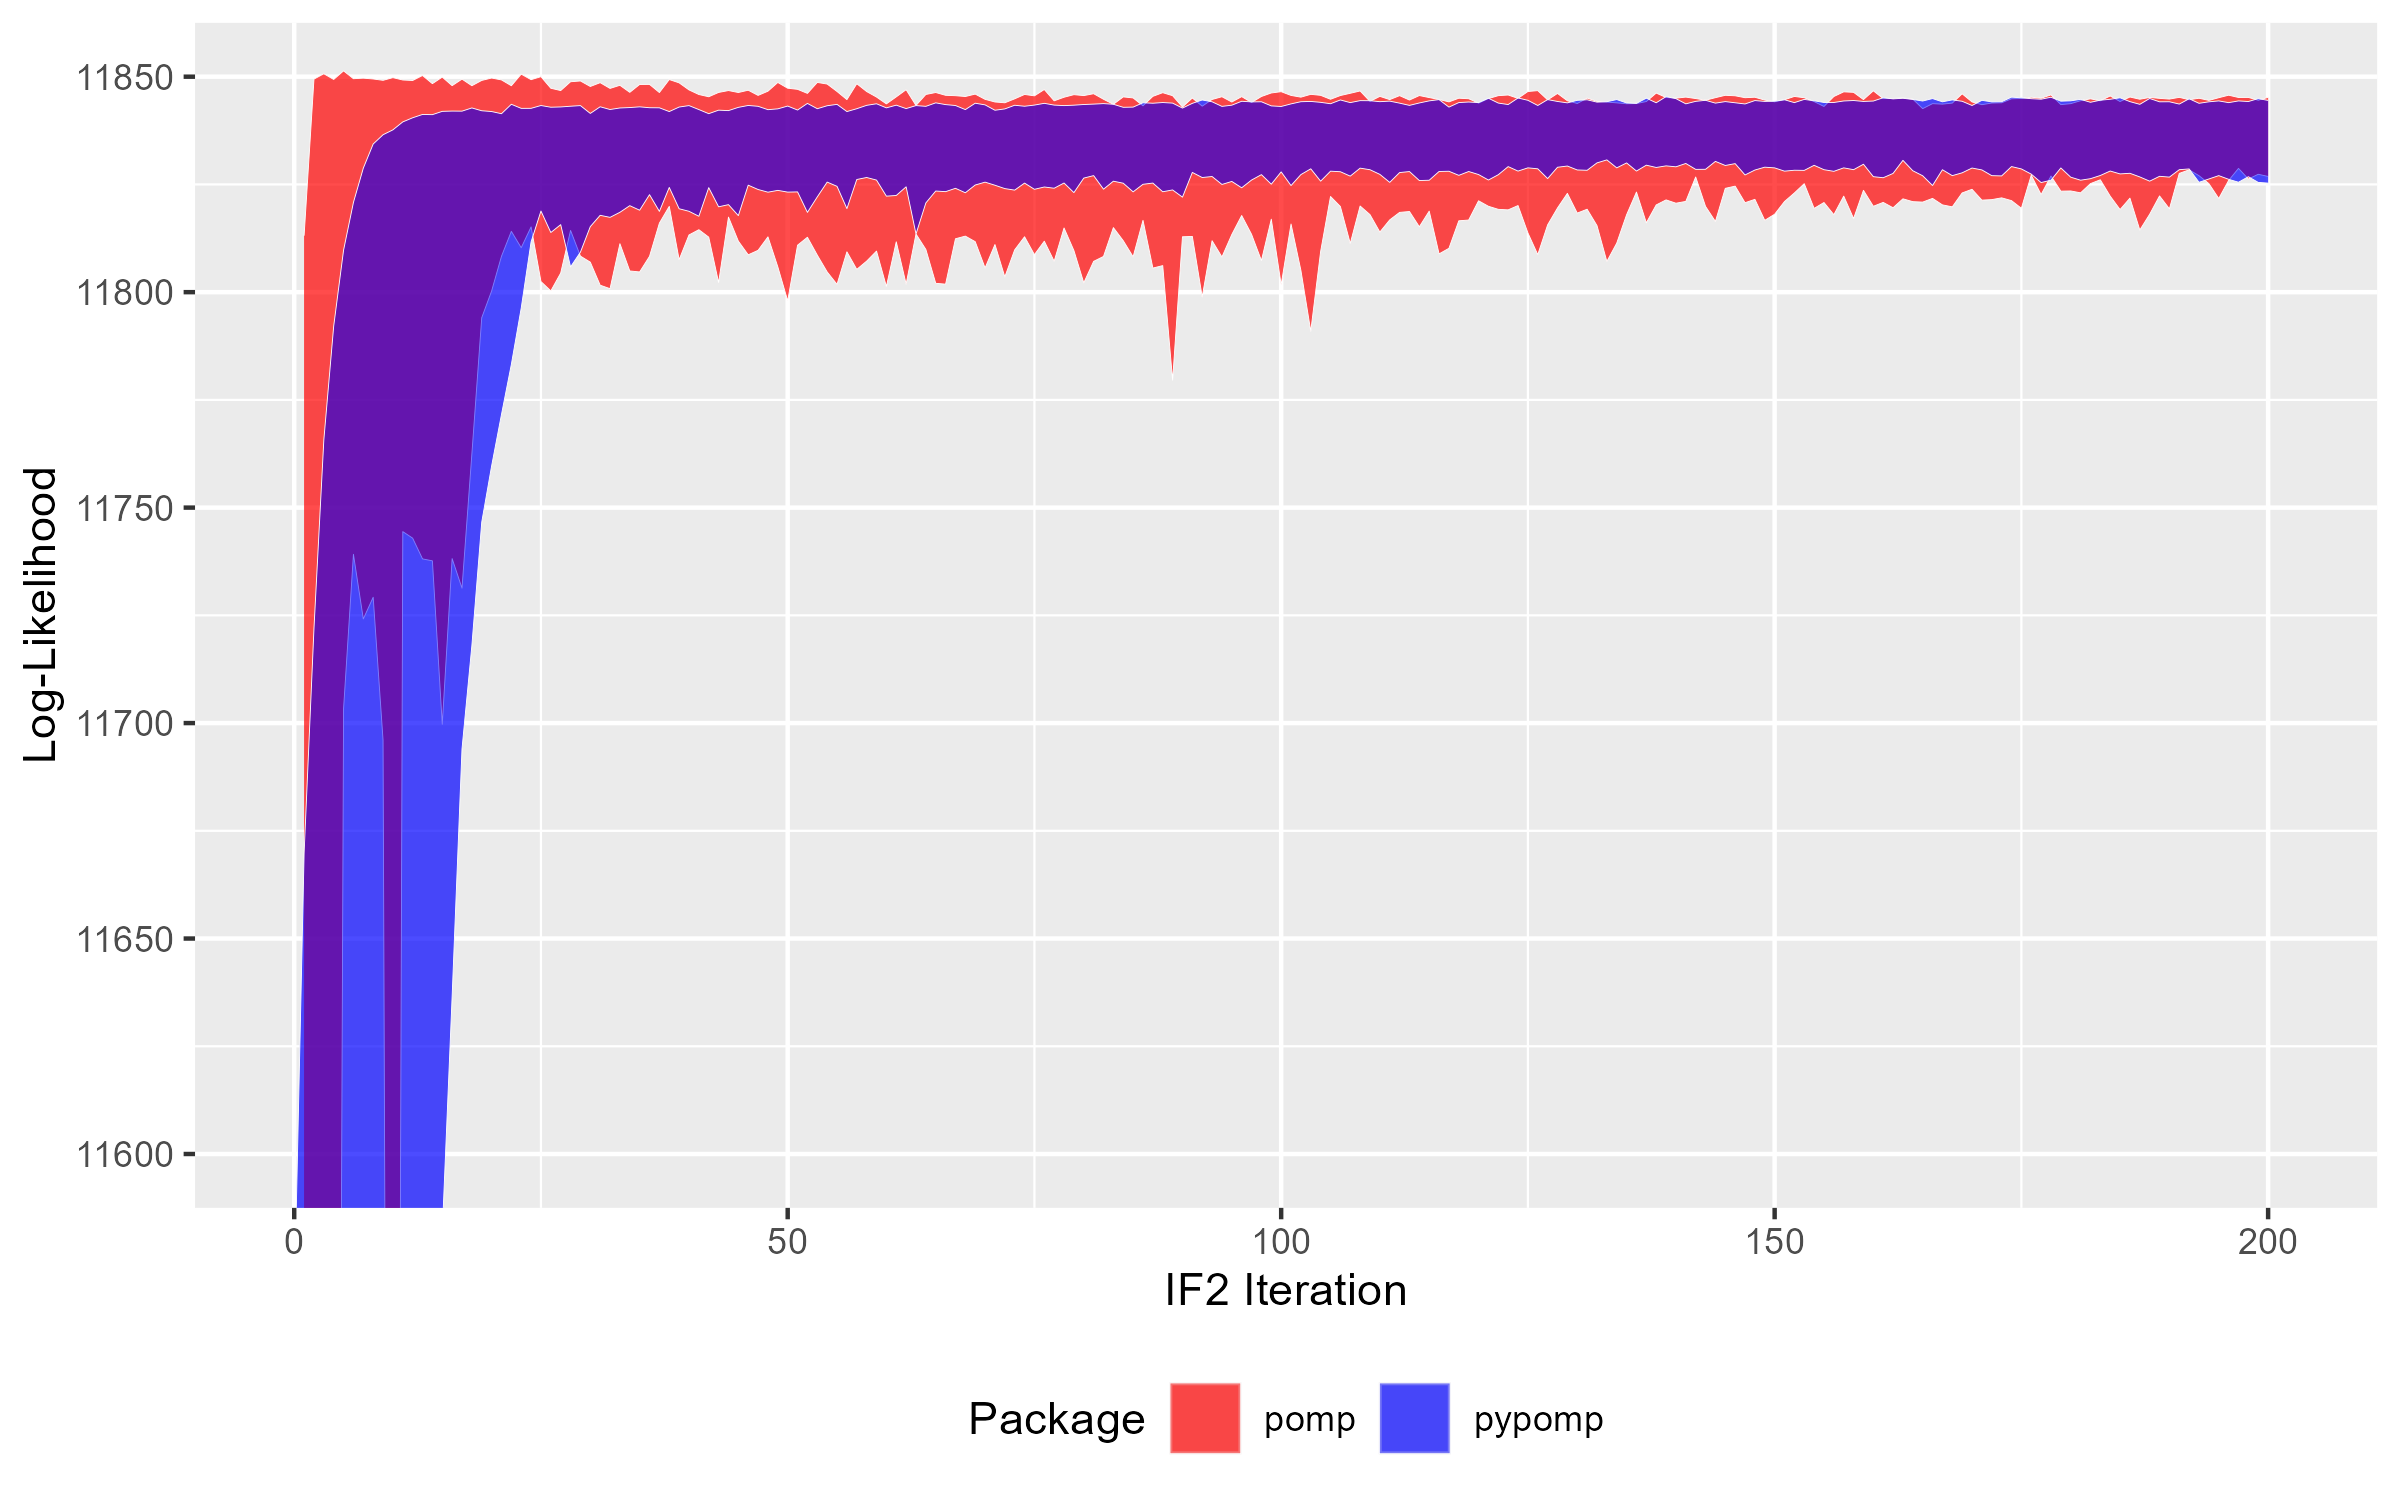
\includegraphics[width=\textwidth]{ll_trace_ribbon_plot.png}
\end{center}
\caption{IF2 Log-Likelihood Trace across Iterations (Outliers excluded)}
\label{fig:if2lltrace}
\end{figure}

Each shaded ribbon in Figure 4.1 represents the 10th–90th percentile range of log-likelihood values across 120 IF2 replicates at each iteration. The values were computed using perturbed parameters at each IF2 iteration and represent noisy estimates of model fit throughout optimization. Although stochastic, the log-likelihood trajectories are expected to improve across iterations as the algorithm converges toward high-likelihood regions.
The results show that broadly similar convergence behavior in both implementations, with \textbf{pypomp} showing noticeably lower variance in its log-likelihood traces compared to \textbf{pomp}. This suggests that \textbf{pypomp} is not exploring the parameter space as extensively as \textbf{pomp}. Thus, while IF2 optimization is functioning and improving log-likelihoods in both packages, there are meaningful differences between the two implementations. Minor differences are always expected when comparing independently developed codebases in different languages, but our findings suggest that \textbf{pypomp}’s IF2 implementation is different from \textbf{pomp} in ways that affect parameter exploration and optimization dynamics and hence could affect the final parameter estimates. 



%%
\section{Parameter Estimate Trace}\label{sec:param_est}
The parameter estimation traces show the evolution of each parameter across IF2 iterations. We average across particles at each iteration to visualize the path of optimization. As parameters are iteratively perturbed and adapted toward the MLE, parameter estimation traces are important in the IF2 process. With this trace, we can analyze whether parameter estimates converge or diverge and whether they exhibit similar dynamics in \textbf{pomp} and \textbf{pypomp}. Also, if both implementations use the same algorithmic parameter values, such as number of particles, number of iterative filtering steps, number of independent IF2 runs from different starting parameter values, number of particle filter evaluation to compute log-likelihood, cooling fraction, random walk standard deviation and starting points, their traces should be similar. This implies that parameter estimation traces provide qualitative assurance between \textbf{pomp} and \textbf{pypomp}.


To assess the consistency of the \textbf{pomp} implementation and the \textbf{pypomp} implementation, we compared the evolution of parameter estimations across IF2 iterations. 


\begin{figure}[ht]
\begin{center}
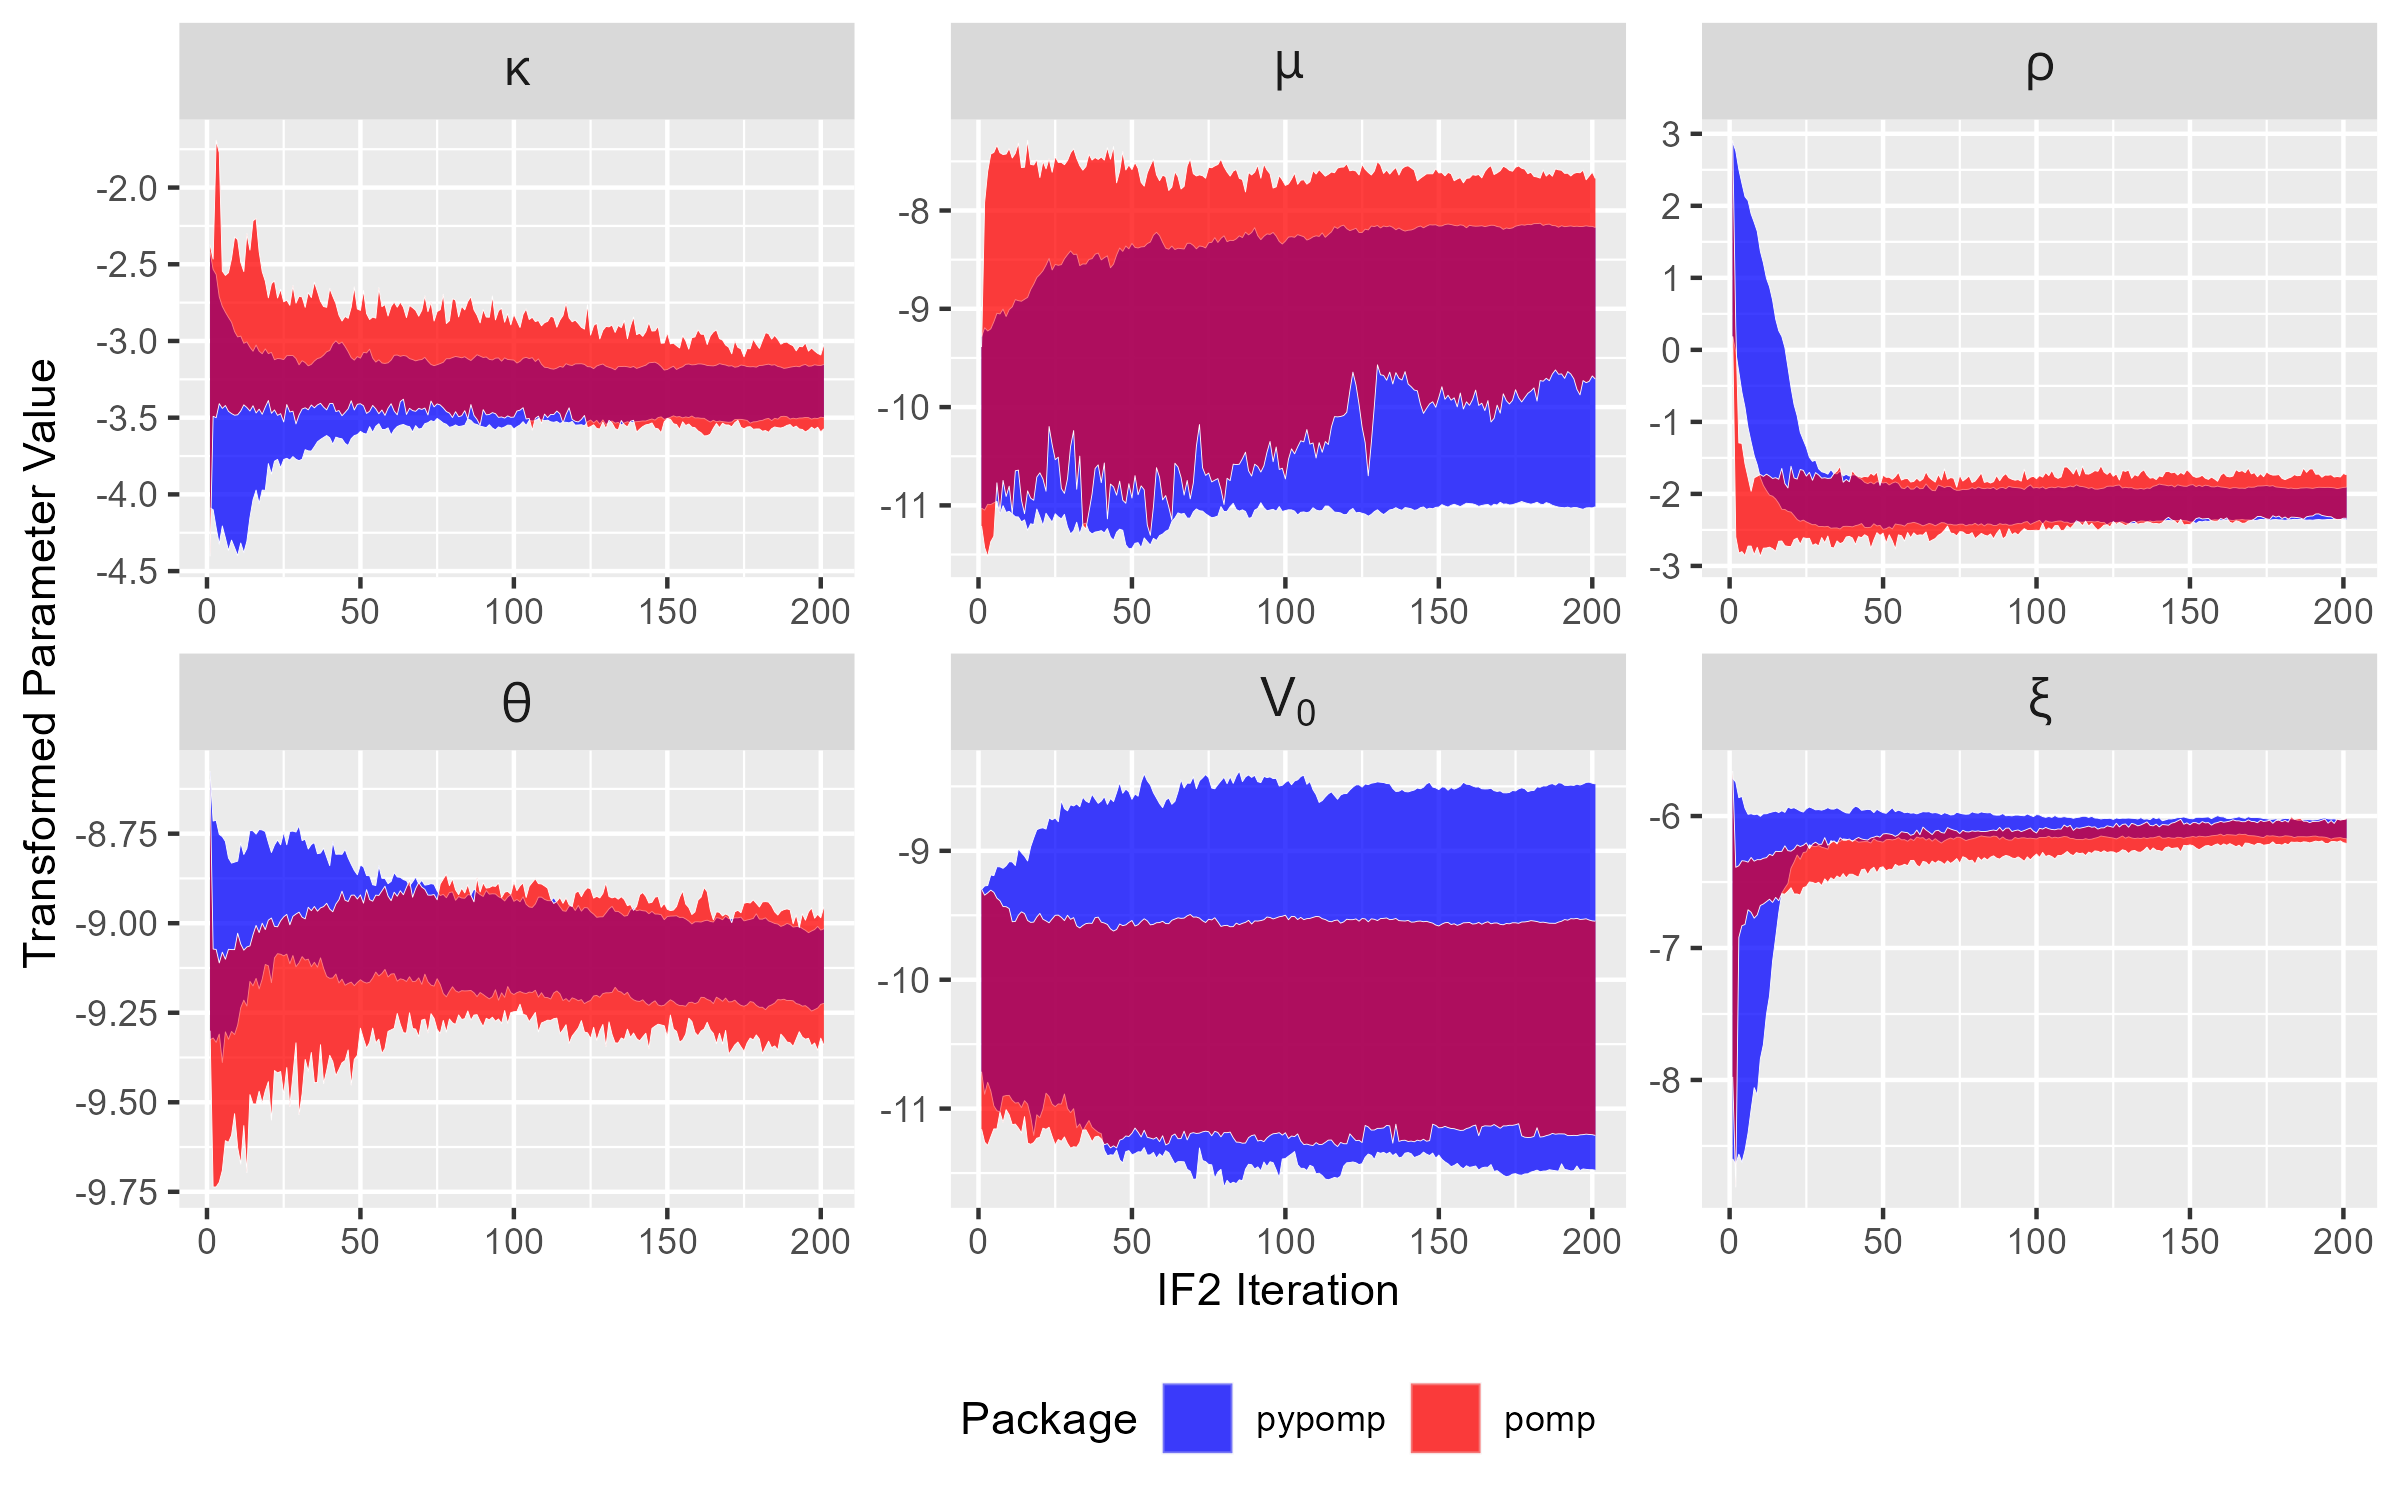
\includegraphics[width=\textwidth]{param_trace_ribbon_plot.png}
\end{center}
\caption{Parameter Estimation Across IF2 Iteration}
\label{fig:if2paramtrace}
\end{figure}

\newpage
Figure 4.2 displays quantile ribbon plots showing the evolution of parameter estimates over IF2 iterations across \textbf{pomp} and \textbf{pypomp} implementations. For each parameter, we show the middle 80\% (10th to 90th percentile) of transformed parameter values at each iteration.
The parameters are transformed to the estimation scale such as log-transformed for positive parameters ($\mu$, $\kappa$, $\theta$, $\xi$, $V_0$) and logit-transformed for the correlation parameter ($\rho$). This transformation ensures a reasonable comparison since both implementations optimize in transformed space. 

Across all six parameters, we observe similar convergence behavior between the two implementations. Both implementations stabilize similarly to transformed values, indicating agreement in the inferred parameter regions but still there are noticeable differences in the median trajectories. 

Then, we assess whether the two implementations arrive at consistent parameter estimate.
\begin{figure}[ht]
\begin{center}
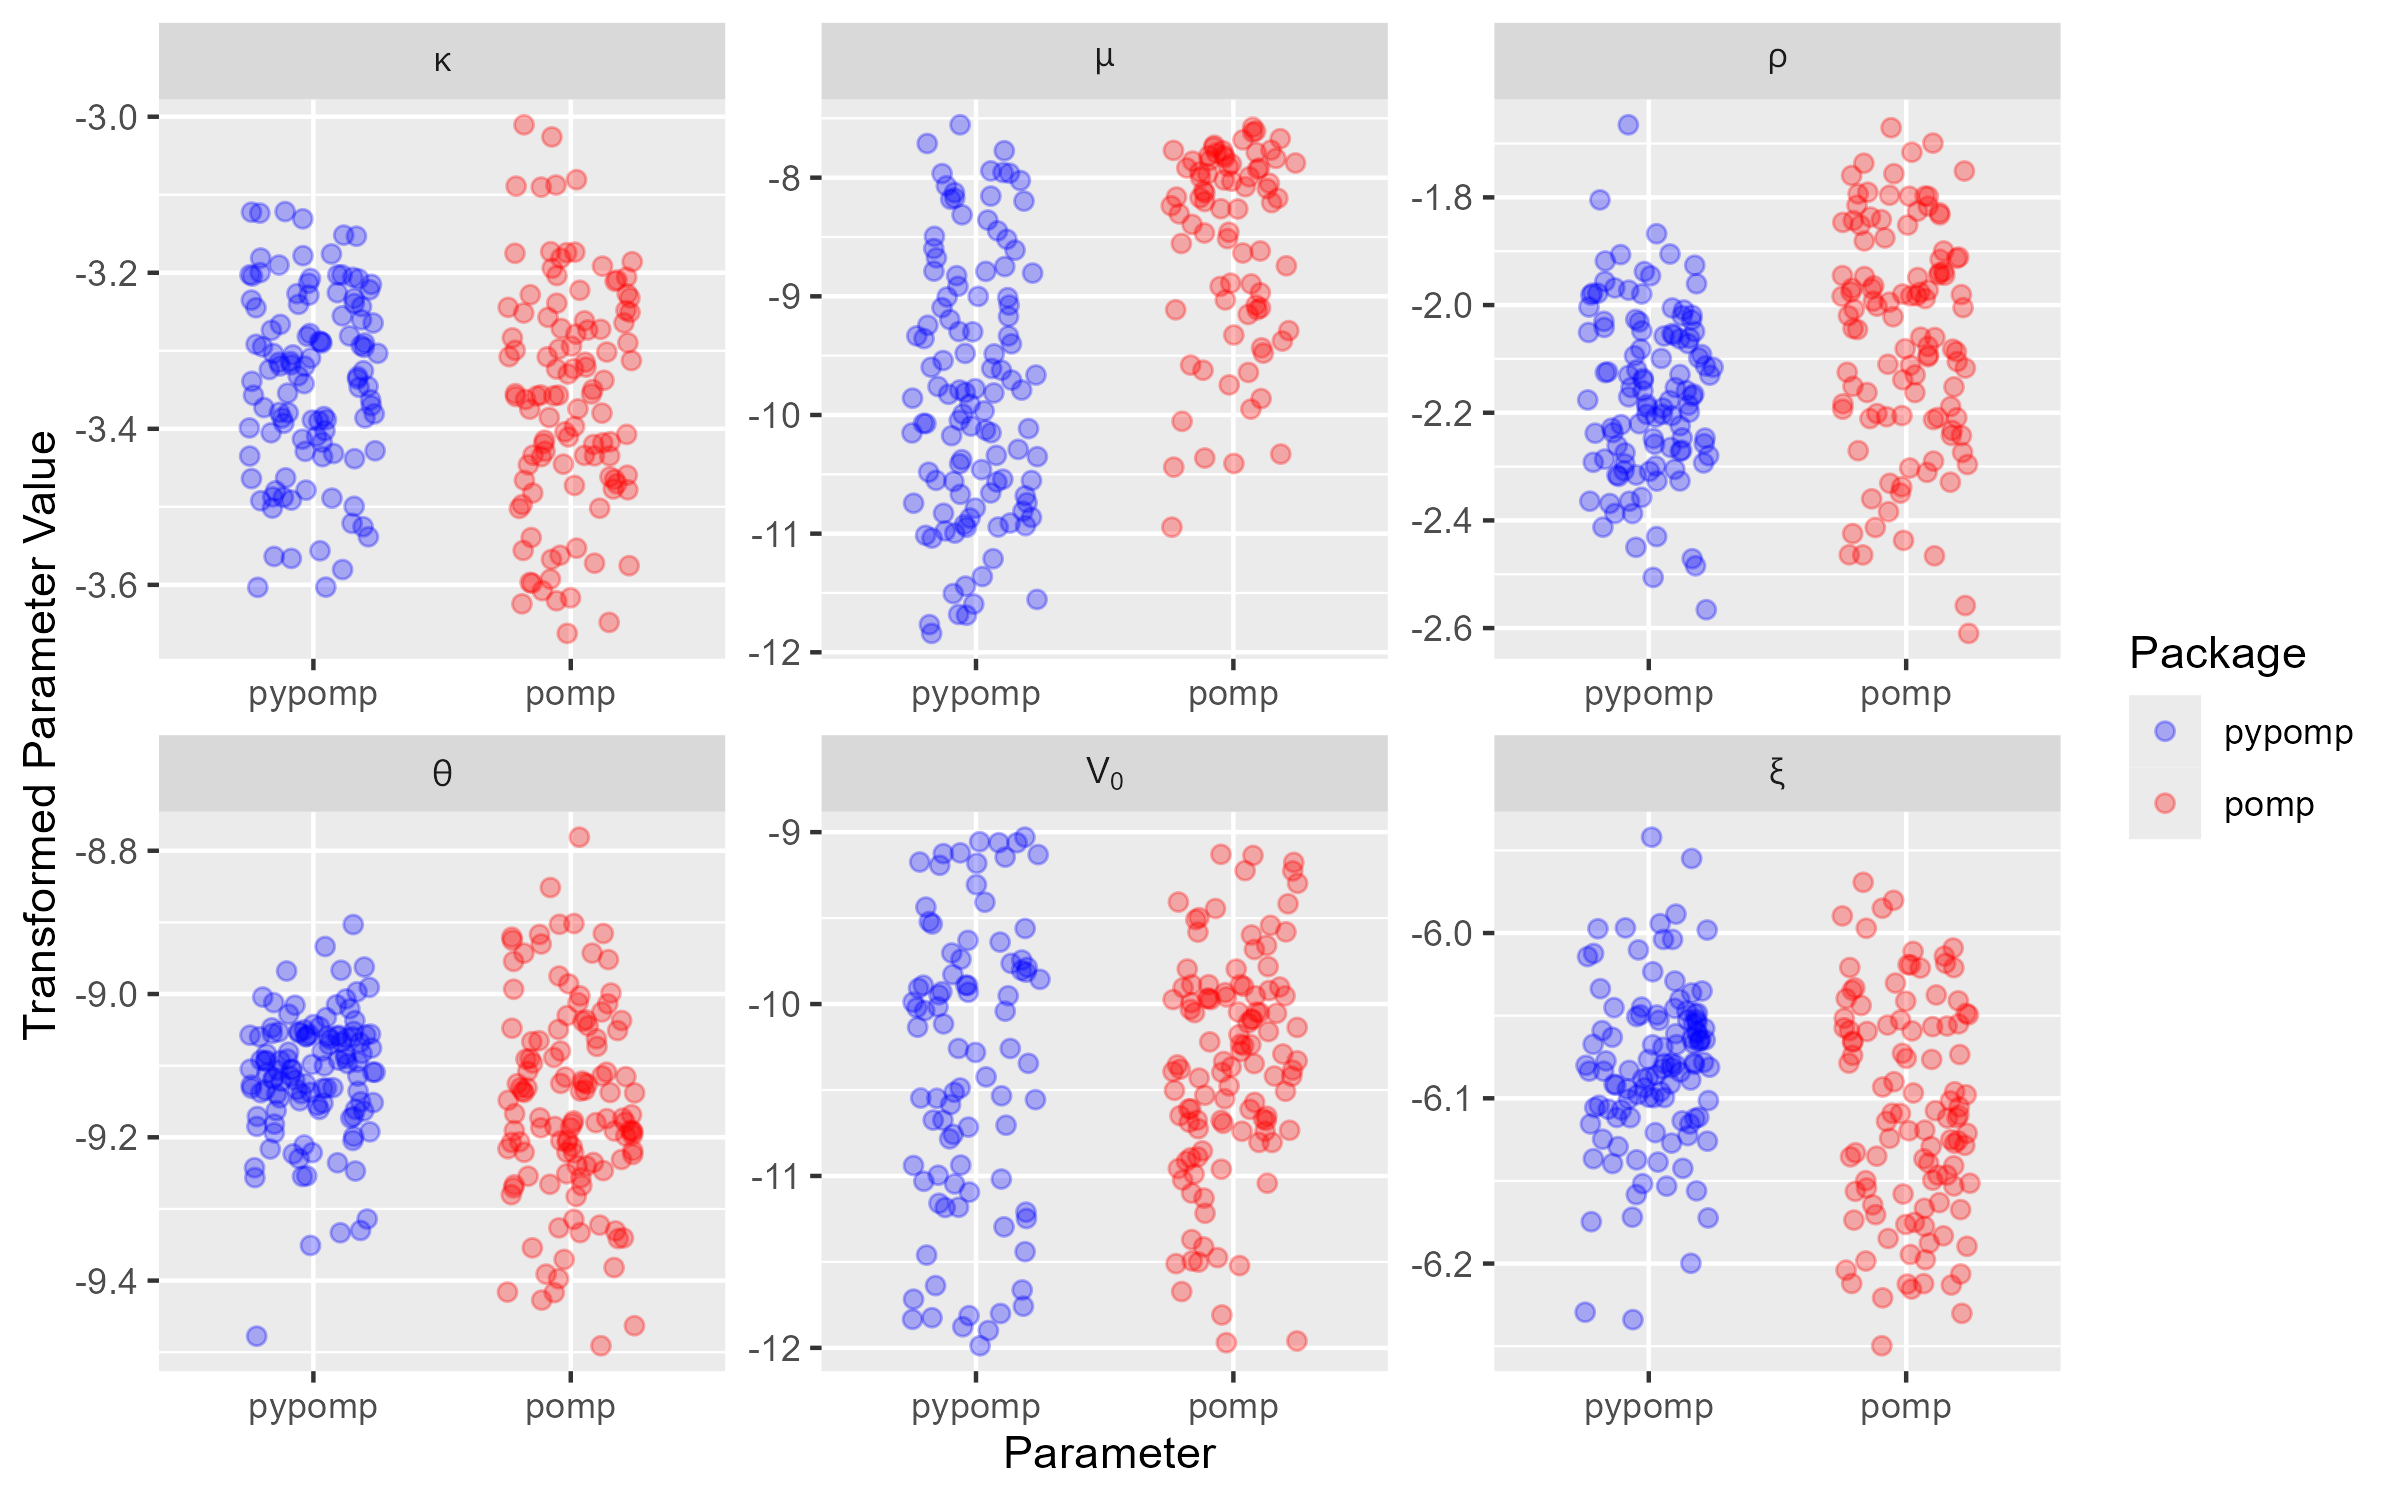
\includegraphics[width=\textwidth]{param_final_iter_plot.png}
\end{center}
\caption{Parameter Estimation at IF2 Final Iteration}
\label{fig:if2paramtrace2}
\end{figure}

\newpage
Figure 4.3 displays the transformed parameter estimates at the final IF2 iteration from 120 independent IF2 runs in both \textbf{pomp} and \textbf{pypomp}. Each point represents the final parameter estimate from one IF2 replicate, transformed to the estimation scale (log or logit). To enhance the interpretability of parameter comparison, extreme parameter estimates were filtered out prior to visualization. For each parameter, we excluded extreme outlier values, corresponding approximately to the lowest and highest 10-30\% of parameter estimates, depending on the distribution. 

Across parameters, the distributions of final estimates are similarly aligned between the two implementations. Slight differences in spread and central tendency appear in $\mu$ and $V_0$ and these results indicate that while the two implementations do not produce identical traces, they broadly agree in terms of convergence region and variability. 

\section{Particle Filter Log-likelihood}\label{sec:pfilter}
After IF2 finishes, the algorithm uses a particle filter with particles and no perturbation to estimate the log-likelihood at the final estimated parameters. For each IF2 run, the algorithm computes the average and standard deviation of estimated log-likelihoods over particle filter replicates. The average log-likelihood assesses the fit quality of the estimated parameters, and the standard deviation gives a sense of Monte Carlo variability.
With these results, given the same number of particles and datasets, IF2 algorithm in both \textbf{pomp} and \textbf{pypomp} yield likelihood estimates with similar accuracy and variability.

To compare the model fit quality across implementations, we examined the log-likelihood values obtained by applying a particle filter to the final parameter estimates from each IF2 run. 
\begin{figure}[ht] 
\begin{center}
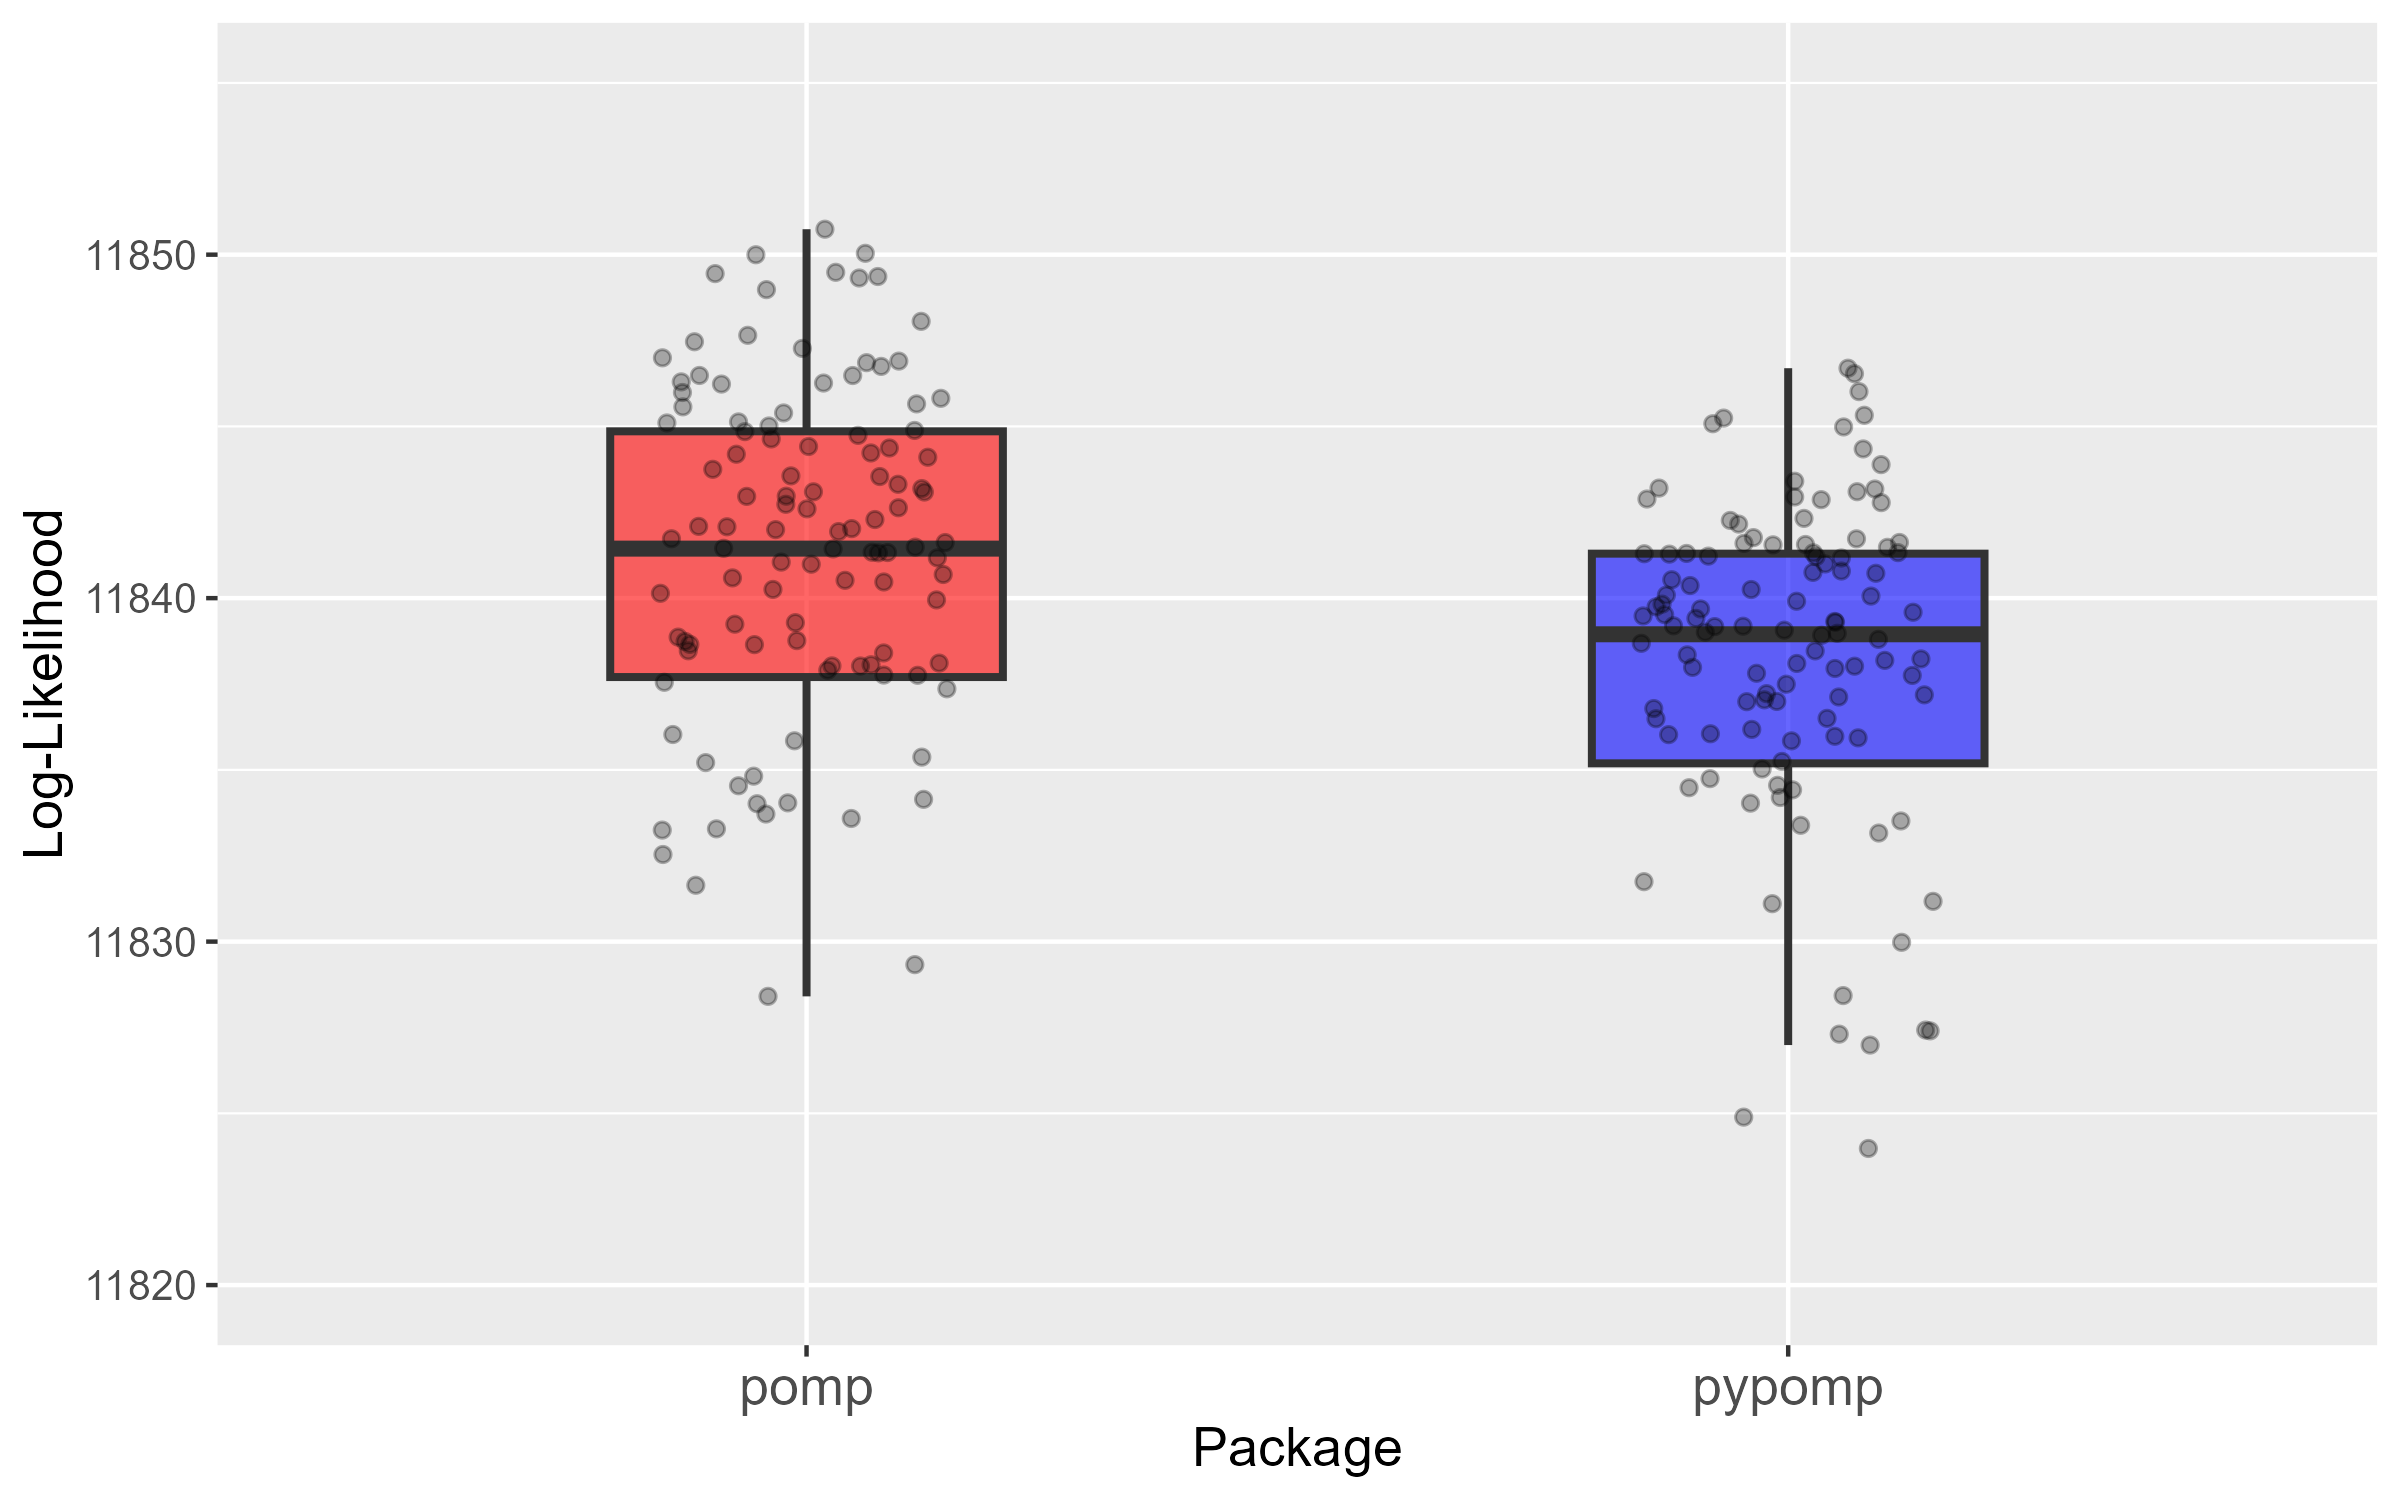
\includegraphics[width=\textwidth]{pfilter_ll_box_plot.png}
\end{center}
\caption{Particle Filter Log-Likelihood at IF2 Final Estimates(Outliers excluded)}
\label{fig:pfilterplot}
\end{figure}

Figure 4.4 shows a comparison of the log-likelihoods from particle filter evaluations at final IF2 estimates across 120 replicates. Each point represents the mean log-likelihood across iterations for one IF2 replicate. While \textbf{pomp} shows a slightly higher median and broader spread with 11850.74 for the highest log-likelihood, \textbf{pypomp} shows lower median and tighter spread with 11847.34 for the highest log-likelihood.

To verify that particle filter in \textbf{pypomp} matches the filter in \textbf{pomp}, we conducted a Monte Carlo-based comparison. Using the same stochastic volatility model and the MLE for each parameter obtained from \textbf{pomp}, we evaluated the log-likelihood using the standard particle filter without parameter perturbation across 24 replicates in \textbf{pypomp}. The best log-likelihood estimated with the MLE in \textbf{pomp} was 11850.74 and the best log-likelihood estimated with the MLE in \textbf{pypomp} was 11848.29 with standard deviation 2.78. These results support the conclusion that the particle filter in \textbf{pypomp} reproduces the behavior of \textbf{pomp} up to expected Monte Carlo variation and the discrepancy between \textbf{pypomp} and \textbf{pomp} stems from the IF2 perturbation step. 

\newpage
\chapter{Automatic Differentiation Particle Filter in pypomp}\label{chap:adpf}
\citet{tan2024accelerated} demonstrate that IFAD outperforms both IF2 and MOP algorithms when applied individually. IF2 alone is prone to slow convergence near the optimum due to diminishing perturbation sizes and MOP alone is sensitive to local minima and saddle points in non-convex likelihood surfaces. The strengths of IFAD are a warm start using IF2 to locate a neighborhood near the MLE and a refinement that uses gradients derived from the MOP-$\alpha$ estimator to perform gradient ascent with AD. This hybrid approach helps IFAD to overcome two critical limitations of IF2 and MOP.

Using the cholera transmission model that developed for Dhaka, Bangladesh \citet{king2008inapparent}, IFAD found log-likelihood values significantly better than those reported using IF2 \citet{ionides2015inference}. Notably, IFAD reaches the MLE with fewer iterations and without the assistance of likelihood profiling. These results indicate IFAD's numerical efficiency and statistical accuracy, and its potential as an innovative plug-and-play method for statistical inference in POMP models.

Encouraged by the numerical efficiency and statistical accuracy of IFAD, we attempted to analyze its performance implemented in \textbf{pypomp} using the Heston stochastic volatility model from \citet{sunmodel}. However, during the implementation and testing of IFAD and MOP in \textbf{pypomp}, we encountered persistent numerical errors and exploding values. Despite initializing the algorithm with plausible parameter values and a reasonable number of particles, errors in gradients and log-likelihoods frequently occurred during the optimization after the first forward mode of AD, suggesting issues within the backward mode of AD execution. As these instabilities do not occur in IF2 implementation of \textbf{pypomp}, it reinforces the conclusion that the source of instability comes from the gradient refinement in MOP implemented in \textbf{pypomp}. 


%%% the third chapter of the main body
\chapter{Discussion}\label{chap:discussion}
Our research contributes to the development, testing, and validation of the early-stage \textbf{pypomp} package. Using the Heston stochastic volatility model as a test case, we examined the behavior and correctness of the IF2 and IFAD algorithms in \textbf{pypomp}, comparing results against \textbf{pomp} package.
For IF2, we demonstrated that \textbf{pypomp} implementation successfully produces log-likelihood estimates and parameter traces that are consistent with the general behavior of IF2. Particle filter process appears to be stable, and likelihood estimates generally improve across iterations, indicating that the core logic of particle filtering and optimization is in place. Despite these promising results, we identified several important discrepancies and design issues that will require attention to ensure that \textbf{pypomp} becomes a fully robust scientific tool.


Although the particle filter behavior matches expectations, there remains meaningful differences between IF2 results from \textbf{pypomp} and \textbf{pomp}, particularly in log-likelihood traces and parameter estimation across iterations. Based on diagnostic comparisons, we conclude that these differences are not due to the particle filter itself, but rather arise from differences in the IF2 perturbation process. Specifically, lower variance in log-likelihood traces of \textbf{pypomp}, compared to \textbf{pomp}, suggests that \textbf{pypomp} may not be exploring parameter space as much as it intended. In addition, a deeper examination of handling random number generation under JAX’s JIT compilation is essential, and PRNG key management must be verified at every stochastic step to ensure true randomness and reproducibility.


For IFAD, although the algorithm is theoretically promising and has shown success in recent research, we encountered persistent numerical instabilities when attempting to apply IFAD to the Heston model in \textbf{pypomp}. These issues include errors in gradients and log-likelihoods, and failures in the optimization after the initial iteration. These issues indicate that while IFAD is a prominent method, the current \textbf{pypomp} implementation should ensure differentiability of the computational graph across all IFAD components and manage numerical stability in weight scaling and normalization, especially in the MOP-$\alpha$ gradient estimators. Beyond debugging, IFAD must be evaluated through quant tests to assess its scalability and practical utility for statistical inference.

Beyond algorithmic issues, several important design considerations were identified during this research. Although the IVP perturbation behavior was corrected during debugging, the fix currently exists in a separate branch and is not yet fully incorporated into the main \textbf{pypomp} IF2 function. Formal integration is necessary to ensure consistent behavior across models. 

On top of that, \textbf{pypomp} currently does not directly provide access to conditional log-likelihoods at each time point within the particle filter. Conditional log-likelihood traces are extremely valuable for model validation and debugging, allowing researchers to identify specific times where model fit deteriorates or where particle depletion occurs. Adding this feature would greatly enhance the transparency and diagnostic functions of \textbf{pypomp}.

At present, \textbf{pypomp} supports IF2, MOP-$\alpha$, and IFAD algorithms but other algorithms available in R \textbf{pomp} such as Particle Markov Chain Metropolis-Hastings algorithm \citep{andrieu2010particle}, and Ensemble Kalman filters \citep{evensen2003ensemble} are not yet implemented. Extending \textbf{pypomp} to include these algorithms would enable broader applicability and make the package a forward compatibility with R \textbf{pomp}.




\newpage


\renewcommand \bibname{Reference}
\addcontentsline{toc}{chapter}{Reference}
%%%\printbibliography
\bibliographystyle{plainnat}
\bibliography{references}
%make citet -> \textcite
\vspace{1cm}
\normalsize



%%% the appendix chapters
\newpage
\appendix
\addcontentsline{toc}{chapter}{Appendix}
\chapter{Algorithms}
%\noindent\textbf{Algorithm 1 IF2} \\[0.5em]
\begin{algorithm}[ht]
\caption{IF2}
\textbf{input:} Simulator for $f_{X_0}(x_0;\theta)$\\
Simulator for $f_{X_n|X_{n-1}}(x_n|x_{n-1};\theta)$, $n$ in $1:N$\\
Evaluator for $f_{Y_n|X_n}(y_n|x_n;\theta)$, $n$ in $1:N$\\
Data, $y_{1:N}^*$\\
Number of iterations, $M$\\
Number of particles, $J$\\
Initial parameter swarm, $\{\Theta_j^0, j$ in $1:J\}$\\
Perturbation density, $h_n(\theta|\varphi;\sigma)$, $n$ in $1:N$\\
Perturbation sequence, $\sigma_{1:M}$\\
\textbf{output:} Final parameter swarm, $\{\Theta_j^M, j$ in $1:J\}$

\begin{algorithmic}[1]
\For{$m$ in $1:M$}
    \State $\Theta_{0,j}^{F,m} \sim h_0(\theta|\Theta_j^{m-1};\sigma_m)$ for $j$ in $1:J$
    \State $X_{0,j}^{F,m} \sim f_{X_0}(x_0; \Theta_{0,j}^{F,m})$ for $j$ in $1:J$
    \For{$n$ in $1:N$}
        \State $\Theta_{n,j}^{P,m} \sim h_n(\theta|\Theta_{n-1,j}^{F,m};\sigma_m)$ for $j$ in $1:J$
        \State $X_{n,j}^{P,m} \sim f_{X_n|X_{n-1}}(x_n|X_{n-1,j}^{F,m}; \Theta_{n,j}^{P,m})$ for $j$ in $1:J$
        \State $w_{n,j}^m = f_{Y_n|X_n}(y_n^*|X_{n,j}^{P,m};\Theta_{n,j}^{P,m})$ for $j$ in $1:J$
        \State Draw $k_{1:J}$ with $\mathbb{P}(k_j = i) = w_{n,i}^m / \sum_{u=1}^J w_{n,u}^m$
        \State $\Theta_{n,j}^{F,m} = \Theta_{n,k_j}^{P,m}$ and $X_{n,j}^{F,m} = X_{n,k_j}^{P,m}$ for $j$ in $1:J$
    \EndFor
    \State Set $\Theta_j^m = \Theta_{N,j}^{F,m}$ for $j$ in $1:J$
\EndFor
\end{algorithmic}
\end{algorithm}

%\noindent\textbf{Algorithm 2 MOP-$\alpha$} \\[0.5em]


\begin{algorithm}[ht]
\caption{MOP-$\alpha$}
\textbf{Input:} Number of particles $J$, timesteps $N$, measurement model $f_{Y_n|X_n}(y_n^*|x_n, \theta)$, simulator process$_n(\cdot|x_n; \theta)$, evaluation parameter $\theta$, baseline parameter $\phi$, seed $\omega$. \\
\textbf{First pass:} Set $\theta = \phi$ and fix $\omega$, yielding $X_{n,j}^{P,\phi}$, $X_{n,j}^{F,\phi}$, $g^{\phi}_{n,j}$. \\
\textbf{Second pass:} Fix $\omega$, and filter at $\theta \neq \phi$: \\
%\hspace*{1em} 
Initialize particles $X_{0,j}^{F,\theta} \sim f_{X_0}(\cdot;\theta)$, weights $w_{0,j}^{F,\theta} = 1$.
\textbf{Initialize } particles ${X}_{0,j}^{F,\theta} \sim {f}_{{X}_{0}}\left(\cdot;{\theta}\right)$, weights $w^{F,\theta}_{0,j}= 1$. \\
%\hspace*{1em} 
%\textbf{For} $n = 1,\ldots,N$ \textbf{do}
\begin{algorithmic}[1]
\For{$n=1,\dots,N$:}
\State Accumulate discounted weights, $w_{n,j}^{P,\theta} = \big(w_{n-1,j}^{F,\theta}\big)^\alpha$.
\State Simulate process model, $X_{n,j}^{P,\theta} \sim \text{process}_n\big(\cdot|{X}_{n-1,j}^{F, \theta};{\theta}\big)$.
\State Measurement density, $g^{\theta}_{n,j}={f}_{{Y}_{n}|{X}_{n}}(y_{n}^{*}|{X}_{n,j}^{P,\theta};{\theta})$.
\State Compute $L_n^{B,\theta,\alpha} ={\sum_{j=1}^Jg^\theta_{n,j} \, w^{P,\theta}_{n,j}}\, \big/\, {\sum_{j=1}^J  w^{P,\theta}_{n,j}}$.
\State Conditional likelihood under $\phi$, $L_n^{\phi} = \frac{1}{J}\sum_{m=1}^{J}g^{\phi}_{n,m}$.
\State Select resampling indices $k_{1:J}$ with $\mathbb{P}\big(k_{j}=m\big) \propto g^{\phi}_{n,m}$.
\State Obtain resampled particles ${X}_{n,j}^{F,\theta}={X}_{n,k_{j}}^{P,\theta}$.
\State Calculate corrected weights $w_{n,j}^{F,\theta}= w^{P,\theta}_{n,k_j} \, g^{\theta}_{n,k_j} \, \big/ \, { g^{\phi}_{n,k_j}}$..
\State Compute $L_n^{A,\theta,\alpha} = L_n^\phi\cdot {\sum_{j=1}^J w^{F,\theta}_{n,j}} \, \big/ \, {\sum_{j=1}^J  w^{P,\theta}_{n,j}}$.
\EndFor
\end{algorithmic}
\textbf{Return:} likelihood estimate $\hat{\mathcal{L}}(\theta) = \prod_{n=1}^N L_n^{A,\theta,\alpha}$ or $\hat{\mathcal{L}}(\theta) = \prod_{n=1}^N L_n^{B,\theta,\alpha}$, filtering distributions $\{(X_{n,j}^{F, \theta}, w^{F,\theta}_{n,j})\}_{n,j=1}^{N,J}$.
\end{algorithm}







%\noindent\textbf{Algorithm 3 IFAD} \\[0.5em]
\begin{algorithm}[ht]
\caption{IFAD}
\textbf{Input:} Number of particles $J$, timesteps $N$, IF2 and MOP-$\alpha$ cooling schedules $\eta_m$, MOP-$\alpha$ discounting parameter $\alpha$, $\theta_0$, $m=0$.
\\
Run initial IF2 search under cooling schedule $\eta_m$ to obtain $\{\Theta_j, j=1,...,J\}$, set $\theta_m := \frac{1}{J}\sum_{j=1}^J \Theta_j$.\\
\textbf{While} procedure not converged:
\begin{algorithmic}[1]
\State Run MOP-$\alpha$ Algorithm to obtain $\hat{\ell}(\theta_m)$.
\State Set $g(\theta_m) := \nabla_{\theta}(-\hat{\ell}(\theta_m))$, and consider any $H(\theta_m)$ such that $\lambda_{\min}(H(\theta_m)) \geq c$.
\State Update $\theta_{m+1} := \theta_m - \eta_m (H(\theta_m))^{-1} g(\theta_m)$, $m := m+1$.
\end{algorithmic}
\textbf{Return} $\hat{\theta} := \theta_m$.
\end{algorithm}

\bigskip

%\newpage
%\chapter{The second appendix}
%A text for appendix 2 starts here.

%%% the index chapter
\newpage
\addcontentsline{toc}{chapter}{Index}
\printindex

\end{document}